\section{Shor-Algorithmus}
Im folgenden Kapitel wird der Shor-Algorithmus zum Faktorisieren von Zahlen beschrieben.
Der Inhalt bezieht sich auf den Zweck, die Funktionsweise und den Aufbau des Algorithmus.
Der Aufbau beinhaltet nicht die konkrete Implementierung der Bestandteile des Algorithmus.
Stattdessen werden die Details bezüglich der Implementierung im nächsten Kapitel behandelt.

\subsection{Zweck}
Der Shor-Algorithmus wurde mit dem spezifischen Ziel entwickelt, 
große zusammengesetzte Zahlen effizient auf Quantencomputern in ihre Primfaktoren zu faktorisieren. 
Im Gegensatz zu klassischen Faktorisierungsverfahren, die exponentielle Zeit erfordern~\cite{katz2023}, 
ermöglicht Shor's Ansatz die Faktorisierung in polynomialer Zeit, 
in Bezug auf die Anzahl an Bits der zu faktorisierenden Zahl~\cite{Shor_1997}. 
Dies stellt eine signifikante Beschleunigung gegenüber den besten bekannten klassischen Faktorisierungsverfahren dar.
Der Shor-Algorithmus bekräftigt die These, das Quantencomputer
bestimmte Probleme wesentlich schneller lösen können als ihre klassischen Gegenstücke.

\subsection{Funktionsweise} \label{Funktionsweise}
Der Shor-Algorithmus verwendet zwei Teilberechnungen, die zusammen die Faktorisierung berechnen.
Die erste Teilberechnung erfolgt mittels eines Quantenalgorithmus. 
Der zweite Teil basiert auf einem klassischen Algorithmus.
Im quantenmechanischen Teil des Shor-Algorithmus geht es um die Bestimmung der Ordnung in der multiplikativen Gruppe modulo \(N\).
Hierbei ist anzumerken, dass der Quantenalgorithmus nicht direkt die Primfaktoren der zu faktorisierenden Zahl berechnet.
Stattdessen wird die Eigenschaft ausgenutzt, 
dass das Problem der Faktorisierung äquivalent zu dem Problem der Ordnungsbestimmung ist~\cite{nielsen_chuang_2010}.
Daher impliziert eine effiziente Lösung für die Berechnung der Ordnung eine ebenso effiziente Methode zur Faktorisierung.
Der nachfolgende klassische Algorithmus verwendet die ermittelte Ordnung, 
um die Primfaktoren abzuleiten. 
Beide Teilberechnungen, sowohl die quantenmechanische als auch die klassische, 
führen ihre Berechnungen in polynomialer Zeit durch. 
Daher liegt die gesamte Laufzeit des Shor-Algorithmus ebenfalls in einer polynomialen Größenordnung.

\subsection{Ordnungsbestimmung} \label{Shor:Ordnungsbestimmung}
Zu bestimmen sind die Primfaktoren der Zahl \(N\).
Zuerst wird ein \(a\) mit \(0 < a < N\) gewählt.
Falls der ungewöhnlichen Fall eintritt, dass \(a\) nicht teilerfremd zu \(N\) ist, entspricht \(a\) einem der Primfaktoren.
Anschließend wird die Ordnung beziehungsweise Periode \(p\) der Funktion \({f(x) = a^x \mod N}\) mit einem Quantenalgorithmus bestimmt:

Die Periode \(p\) beschreibt das kleinste ganzzahlige Element mit \({p > 0}\), für das gilt: \({f(p) = 1 \mod N}\).
\[
\begin{tabular}{l|llllll}
    x     &     0     &     1       &     2      &      3   &  4 &  5  \\ \hline
    \(7^x \mod 15\)    &      1     &        7     &       4     &     13     &  1 &  7 
\end{tabular} \longmapsto p = 4
\]

Im Wesentlichen handelt es sich bei der quantenmechanischen Berechnung des Shor-Algorithmus um die Quanten-Phase-Estimation.
Die Architektur dieser spezifischen Quanten-Phase-Estimation korrespondiert weitgehend mit der in Abschnitt~\ref{Quanten-Phase-Estimation} vorgestellten Struktur.
Hierbei ersetzen speziell für die gegebene Anwendung definierte \(U\)-Gatter die allgemeinen.

Für den konkreten Kontext der Periodenberechnung, realisieren die \(U\)-Gatter die Transformation:
\[U\ket{y} = \ket{ay \mod N}\] 
Die Ausführung der Quanten-Phase-Estimation erfordert die Erzeugung eines Eigenvektors der Transformation \(U\).
Da die Quanten-Phase-Estimation \(\varphi\) aus dem Eigenwert extrahiert, 
darf der Eigenvektor nicht den trivialen Eigenwert 1 besitzen.
Stattdessen ist es notwendig, dass die Periode der Transformation im Eigenwert enthalten ist.

Wie in~\autocite[227]{nielsen_chuang_2010} gezeigt wird, gibt es zu \(U\) Eigenvektoren \(\ket{u_s}\), 
mit \(0 \leq s \leq p-1\): 
\[\ket{u_s} \equiv
\frac{1}{\sqrt{p}}
\sum_{k=0}^{p-1} e^{\frac{-2 \pi i s k}{p}\ket{a^k \mod N}} %ich soll die Formel mit der Summe sein
\]
Für \(a=7\) bei \(N=15\) entspricht \(r=4\).
Ein Eigenvektor zu \(s=1\) lautet dann:
\[
    \ket{u_1}_4 =
    \frac{1}{\sqrt{4}}(
        \ket{1}_4 + 
        e^{-\frac{2 \pi i}{4}}\ket{7}_4 + 
        e^{-\frac{4 \pi i}{4}}\ket{4}_4+ 
        e^{-\frac{6 \pi i}{4}}\ket{13}_4
    )
    \]
\[
    U\ket{u_1}_4 =
    \frac{1}{\sqrt{4}}(
        \ket{7}_4 + 
        e^{-\frac{2 \pi i}{4}}\ket{4}_4 + 
        e^{-\frac{4 \pi i}{4}}\ket{13}_4+ 
        e^{-\frac{6 \pi i}{4}}\ket{1}_4
    )
    \]
\[
    U\ket{u_1}_4 =
    e^{\frac{2 \pi i}{4}}
    \cdot
    \frac{1}{\sqrt{4}}(
        e^{-\frac{2 \pi i}{4}}\ket{7}_4 + 
        e^{-\frac{4 \pi i}{4}}\ket{4}_4 + 
        e^{-\frac{6 \pi i}{4}}\ket{13}_4+ 
        e^{-\frac{8 \pi i}{4}}\ket{1}_4
    )
    \]
\[
    U\ket{u_1}_4 =
    e^{\frac{2 \pi i}{4}}
    \cdot
    \frac{1}{\sqrt{4}}(
        e^{-\frac{8 \pi i}{4}}\ket{1}_4
        e^{-\frac{2 \pi i}{4}}\ket{7}_4 + 
        e^{-\frac{4 \pi i}{4}}\ket{4}_4 + 
        e^{-\frac{6 \pi i}{4}}\ket{13}_4 )
    =
    e^{\frac{2 \pi i}{4}} \cdot
    \ket{u_1}_4
    \]
Das kann verallgemeinert werden:
\[U\ket{u_s} = e^{\frac{2 \pi i s}{p}}\ket{u_s}\]

Wie man in der Definition von \(\ket{u_s}\) %ref zu Formel mit der Summe
sieht, 
benötigt die Initialisierung eines Eigenvektors \(\ket{u_s}\) mit einem konkreten \(s\) die Periode \(p\).
Man kann diese Problematik jedoch umgehen indem man anstelle eines einzelnen Eigenvektors \(\ket{u_s}\)
eine Superposition verwendet, die alle \(\ket{u_s}\) umfasst.
Die Superposition entspricht~\autocite[227]{nielsen_chuang_2010}:
\[\frac{1}{\sqrt{p}} \sum_{s=0}^{r-1}\ket{u_s} = \ket{1}\] 
Also wird das Qubit, welches das Least-Significant-Bit des für den Eigenvektor bestimmten Qubit-Registers repräsentiert, 
mit \(\ket{1}\) initialisiert.

Die Superposition der Eigenvektoren hat zur Folge, 
dass nach der inversen Quanten-Fourier-Transformation, also am Ende der Quanten-Phase-Estimation,
ebenfalls eine Superposition mit dem \(\varphi_s\) der Eigenwerte \(\lambda_{u_s}\) aller möglichen Eigenvektoren \(\ket{u_s}\) existiert.
Sei \(k\) die Anzahl an Kontroll-Qubits dann:
\[
    \frac{1}{\sqrt{p}} \sum_{s=0}^{p-1}\ket{2^k \cdot \frac{s}{p}}_k   = 
    \frac{1}{\sqrt{p}} (\ket{0}_k  + \ket{2^k \cdot \frac{1}{p}}_k + \ket{2^k \cdot \frac{2}{p}}_k  ... + \ket{2^k \cdot \frac{p-1}{p}}_k )
    \]


Bei einer Messung wird also zufällig eines der insgesamt \(p\) vielen \(\varphi_s \approx \frac{s}{p}\) gemessen.

Die Genauigkeit des Algorithmus, ausgedrückt durch den Parameter \(k\),
ist direkt abhängig von der Anzahl der verwendeten \(U^{2^x}\)-Gatter
und der damit assoziierten Kontroll-Qubits im Quantenschaltkreis.
Die Genauigkeit des Messergebnisses gegenüber dem \(\varphi_s\) hängt von \(k\) ab.

Wenn genügend Kontroll-Qubits verwendet werden, 
wird bei einer Messung ein Zustand gemessen, 
in welchem \(\frac{s}{p}\) enthalten ist.

Falls nicht ausreichend Kontroll-Qubits vorhanden sind 
und der Wert von \(\varphi_s\) somit nicht ausreichend umfasst werden kann,
wird die Messung mit hoher Wahrscheinlichkeit 
in einen der möglichen Zustand kollabieren, 
der dem genauen Ergebnis am nächsten ist. 
Dadurch bilden sich ein Peak rund um den korrekten Wert, 
welcher Vergleichbar ist mit Abbildung~\ref{fig:3_qubit_qpe_measurment_uncertain}.
Genau wie in Abbildung~\ref{fig:3_qubit_qpe_measurment_uncertain}, haben die Werte nah dem genauen Wert
eine höhere Chance gemessen zu werden. 
Da aber eine Messung von probabilistischer Natur ist, 
kann eine Messung auch zu einem Ergebnis führen, 
welches entfernt vom genauen Ergebnis liegt.

Anders als in Abbildung~\ref{fig:3_qubit_qpe_measurment_uncertain} gibt es bei der Periodenbestimmung insgesamt \(p\) Peaks.
Das liegt daran, dass es insgesamt \(p\) viele Zustände in der Superposition des Endzustandes gibt.

Anhand des Messergebnisses erfolgt die Primfaktorzerlegung in einer Nachberechnung.

\subsection{Klassische Nachberechnung} \label{Funktionsweise:klassisch}
Die Nachberechnung benötigt keine Quantenbrechnung und 
wird somit mit einem klassischen Algorithmus durchgeführt.

Ein einzelner Zustand der finalen Superposition, 
entspricht einem genauen Ergebnis und besitzt die Form \(\ket{2^k \cdot \frac{s}{p}}_k\) für \(0 \leq s < p\).
Mit einer Division durch \(2^k\) kann \(\frac{s}{p}\) extrahiert werden.
Zum Beispiel ist die finale Superposition für \(a = 7;~N=15\) mit \(p=4\) bei einer Genauigkeit \(k=4\):
\[\frac{1}{\sqrt{4}}(\ket{0}_4 +\ket{2^4 \cdot \frac{1}{4}}_4 + \ket{2^4 \cdot \frac{2}{4}}_4+\ket{2^4 \cdot \frac{3}{4}}_4) =
 \frac{1}{\sqrt{4}}(\ket{0}_4 +\ket{4}_4 + \ket{8}_4+\ket{12}_4) \]
Mit Ausnahme der Zustände \(\ket{0}_4\) und \(\ket{8}_4\), 
gewähren die beiden anderen Zustände nach einer Division mit \(2^4\) eine Kommazahl, 
die als Bruch die gesuchte Periode \(p=4\) als Nenner enthält.

Im vorherigen Beispiel handelt es sich bei der Periode um eine 2er Potenz, 
weswegen die Messergebnisse eindeutig sind.
Jedoch ist dies ein ideales Szenario welches bei immer größeren \(N\) seltener auftretet. 
Das nächste Beispiel beachtet \(a=11;~N=21\) mit der Periode \(p=6\) bei einer Genauigkeit \(k=4\):
\[\frac{1}{\sqrt{6}}(\ket{0}_4 +\ket{2^4 \cdot \frac{1}{6}}_4 + \ket{2^4 \cdot \frac{2}{6}}_4+
\ket{2^4 \cdot \frac{3}{6}}_4)+\ket{2^4 \cdot \frac{4}{6}}_4 + \ket{2^4 \cdot \frac{5}{6}}_4 \]
\[= \frac{1}{\sqrt{6}}(\ket{0}_4 +\ket{2,\overline{6}}_4 + \ket{5,\overline{3}}_4+
\ket{8}_4+\ket{10,\overline{6}}_4 + \ket{13,\overline{3}}_4) \]
Die Kontroll-Qubits, welche gemessen werden, 
können keine Kommazahlen darstellen.
Als Folge davon, bildet sich um die benachbarten Zustände eine Wahrscheinlichkeitsverteilung, 
die bei dem ganzzahligen Zustände, der am nächst liegt, ihren Hochpunkt hat,
vergleichbar mit~\ref{fig:3_qubit_qpe_measurment_uncertain}.
Im konkreten Beispiel wird für \(\ket{2,\overline{6}}_4\) der Zustand \(\ket{3}_4\) 
mit der höchsten Wahrscheinlichkeit gemessen.
Eine Extraktion der Periode aus \(\ket{3}_4\)  mit \(\frac{3}{2^4}\) liefert als Ergebnis die Kommazahl \(0,1875\).
Mit dem Kettenbruch-Algorithmus wird zu der Kommazahl der nächstgelegene Bruch gefunden, 
im konkreten Fall die \(\frac{3}{16}\).
Der Bruch \(\frac{3}{16}\) enthält im Nenner nicht die gesuchte Periode \(p=6\). 
Das Gleiche gilt auch für andere Zustände, 
die mit hoher Wahrscheinlichkeit gemessen werden können, wie 
\(\ket{5}_4,~\ket{8}_4,~\ket{11}_4\) und \(\ket{13}_4\).

Das Versagen der vorausgegangenen Berechnung ist auf eine unzureichende Genauigkeit zurückzuführen. 
In der vorangegangenen Darstellung werden \(k=4\) Kontroll-Qubits eingesetzt, 
welche für die gesuchte Periode einen zu kleinen Wertebereich bilden.

Wiederholt man das ganz, mit \(k=7\), erhält man folgende Superposition:
\[\frac{1}{\sqrt{6}}(\ket{0}_7 +\ket{21,\overline{3}}_7 + \ket{42,\overline{6}}_7+
\ket{64}_7+\ket{85,\overline{3}}_7 + \ket{106,\overline{6}}_7) \]
Es ist ersichtlich, dass die genauen Zustände weiterhin über Nachkommastellen verfügen.
Weswegen mit einer geringeren Wahrscheinlichkeit auch andere Werte gemessen werden können.
Bei einer Messung ist statt des Zustands \(\ket{21,\overline{3}}_7\) der Zustand \(\ket{21}_7\) das wahrscheinlichste Ergebnis.
Für \(\frac{21}{2^{7}}\) erhält man eine Kommazahl, deren genauer Bruch \(\frac{21}{128}\) entspricht.
Bekanntlich entspricht die Periode jedoch einer Zahl \(p\) die kleiner ist als \(N\).
Wendet man auf \(\frac{21}{128}\) den Kettenbruch-Algorithmus an und limitiert den Nenner auf \(N\), 
wird der nächstgelegene Bruch gefunden, welcher ein Nenner besitzt, der kleiner ist als \(N\).
Im konkreten Beispiel folgt für \(\frac{21}{128}\) der Bruch \(\frac{1}{6}\), 
welcher die Periode im Nenner offenbart.
Bei einer Messung kann auch der benachbarte ganzzahlige Zustand \(\ket{22}_7\) gemessen werden, 
allerdings mit einer geringeren Wahrscheinlichkeit im Vergleich zu \(\ket{21}_7\).
Der Zustand \(\ket{22}_7\) ermöglicht nicht die Extraktion der Phase, 
da \(\frac{22}{128}\) mit dem Kettenbruch-Algorithmus auf einen für \(N\) limitierten Nenner
zu \(\frac{3}{17}\) wird.

Bedeutet mit einer hinreichenden Genauigkeit, kann die Periode nur aus dem Zustand extrahiert werden, 
welcher den Wert des genauen Zustandes am besten approximiert.

Mit zusätzlichen Kontroll-Qubits wird das Messergebnis Fehlertolerant.
Wiederholt man das Beispiel erneut, diesmal jedoch mit \(k=10\), 
ist der zweite Zustand in der finalen Superposition: 
\(\ket{2^{10} \cdot \frac{1}{6}}_{10} =\ket{170,\overline{6}}_{10}\).
Im Gegensatz zu vorher liefert jetzt nicht nur das am besten approximierte Ergebnis, 
in dem Fall die \(\ket{170}_{10}\), mit dem Kettenbruch-Algorithmus die Periode, 
sondern auch alle benachbarten Zustände von \(\ket{167}_{10}\) bis \(\ket{175}_{10}\).

Durch den Einsatz von zusätzlichen Kontroll-Qubits erhöht sich der Wertebereich. 
Aufgrund des größeren Wertebereiches existieren mehr mögliche Zustände, 
die bei einer Messung vorkommen könnten und ebenfalls auch mehr Zustände, 
die die Extraktion der korrekten Periode ermöglichen. 
Dabei ist die Wahrscheinlichkeitsverteilung der ausschlaggebende Faktor. 
Diese verändert sich mit einer wachsenden Anzahl an Kontroll-Qubits zugunsten der Zustände, 
welche die korrekte Periode offenbaren.
Die Abbildungen~\ref{fig:Messung7k} und~\ref{fig:Messung10k} 
heben den Effekt zusätzlicher Kontroll-Qubits auf die Wahrscheinlichkeitsverteilung der Messungen hervor.
Die grünen Säulen im Diagram zeigen die Messergebnisse, welche die Extraktion der Periode erlauben.

\begin{figure} [H]
    \caption{Messergebnisse für a=11, N=21, k=7 bei 1024 Messungen}
    \label{fig:Messung7k}
    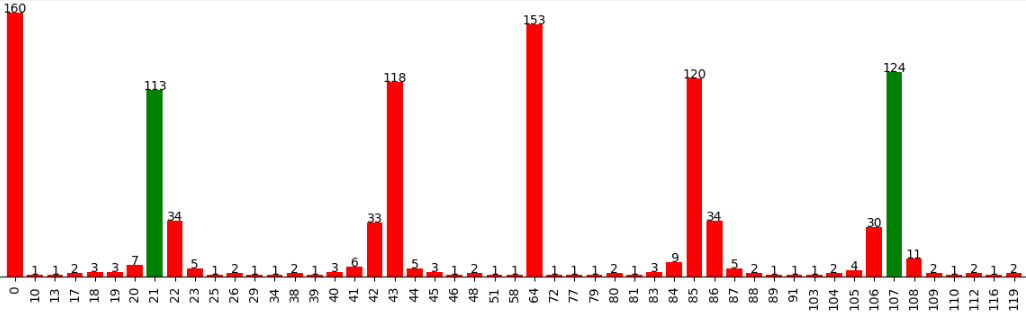
\includegraphics[scale = 0.55]{wahrscheinlichkeit_k7.PNG}
    \centering
    \end{figure}
\begin{figure} [H]
    \caption{Messergebnisse für a=11, N=21, k=10 bei 1024 Messungen}
    \label{fig:Messung10k}
    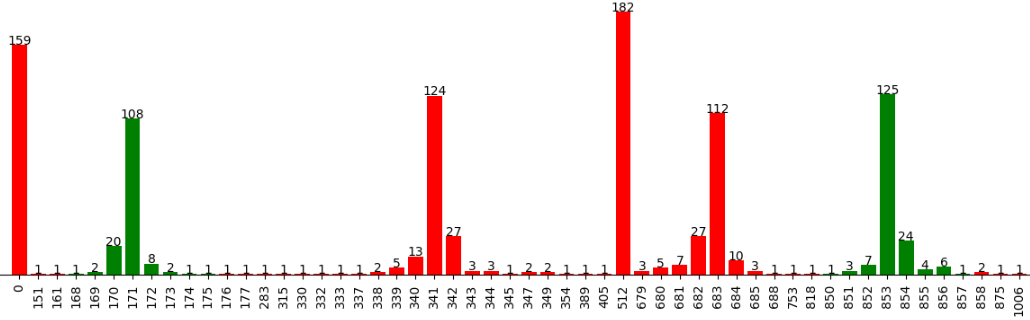
\includegraphics[scale = 0.55]{wahrscheinlichkeit_k10.PNG}
    \centering
    \end{figure}

Für eine bekannte Periode, 
kann man zeigen, 
dass die Verwendung von \(k > 2\text{ld}(p)\) eine ausreichende Genauigkeit liefert,
so dass ein Messergebnis unter Verwendung des Kettenbruch-Algorithmus zu einem Näherungsbruch \(\frac{s}{p}\) von \(\varphi_s\) konvergiert~\cite{Shor_1997}.
Im Normalfall kann für eine Elementes \(a\) für den Modulus \(N\) vorab nicht gesagt werden, 
wie viele Kontroll-Qubits man exakt braucht, 
da dies von der unbekannten Periode \(p\) abhängt.
Stattdessen, verwendet man einen Wert der auf alle Fälle größer als \(2\text{ld}(p)\) ist, 
wie zum Beispiel \(2\text{ld}(N)\)~\cite{Shor_1997}\cite{mosca1999hidden}. 

Wie man in Abbildungen~\ref{fig:Messung10k} sieht, 
gibt es auch bei der Verwendung von \(2\text{ld}(N)\) Kontroll-Qubits drei Szenarien, 
bei denen eine Zustand mit einer ungültigen Periode gemessen werden kann.

Im Falle des ersten Szenarios, 
entspricht mindestens einer der Zustände der finalen Superposition einer Kommazahl.
Dadurch kann es zu Messungen von falschen Werten kommen.
Anhand dieses Ergebnisses führt der Kettenbruch-Algorithmus nicht zu \(\frac{s}{p}\), 
weswegen eine neue Messung benötigt wird.

Das zweite Szenario ähnelt dem ersten und tritt ebenfalls auf, 
sobald mindestens einer der Zustände der finalen Superposition eine Kommazahl ist. 
Im Unterschied zum ersten Szenario liegt dieses Messergebnis jedoch nah bei einem Peak, 
also in der Nähe eines Messergebnisses, aus dem die Periode extrahiert werden kann. 
Indem man die Nachbarzustände des Messergebnisses testet, kann man gegebenenfalls einen Zustand finden, 
der die Extraktion der Periode ermöglicht.

Das zweite Szenario tritt beispielsweise für das Messergebnis \(\ket{176}_{10}\) in Abbildung~\ref{fig:Messung10k} auf.
Die Anwendung des Kettenbruch-Algorithmus auf \(\frac{176}{2^{10}}\) 
liefert nicht die korrekte Periode, stattdessen ergibt sich der Bruch \(\frac{3}{17}\). 
Anstatt eine neue Messung durchzuführen,
ist es in diesem Fall zielführend, 
die ganzzahligen Nachbarn des Messergebnisses zu überprüfen.
Im konkreten Beispiel ermöglicht bereits die geringfügige Anpassung des Messergebnisses durch Subtraktion von 1, 
also zu \(\ket{175}_{10}\), 
die erfolgreiche Extraktion der Periode.

Die Erhöhung der Genauigkeit \(k\) auf Werte über \(2\text{ld}(N)\) hinaus hat den Effekt, 
dass die Wahrscheinlichkeit für das Eintreten des ersten oder zweiten Falls abnimmt.
Dadurch verbessern sich gleichzeitig die Wahrscheinlichkeit, direkt ein korrektes Ergebnis zu messen.
Allerdings führt dies zu einem komplexeren Quantenschaltkreis und 
somit erhöhen sich die Kosten an zusätzlichen Ressourcen~\autocite[231]{nielsen_chuang_2010}.

Der dritte und letzte Fall kann immer auftreten.
In diesem Szenario wird ein \(\frac{s'}{p'}\) gemessen, 
welches entsteht, wenn \(s\) und \(p\) einen gemeinsamen Teiler haben und 
deswegen von \(\frac{s}{p}\) auf \(\frac{s'}{p'}\) gekürzt wurden.
In diesem Fall kann ein vielfaches von \(p'\), also \(2p'\),\(3p'\),.. zum richtigen \(p\) führen.
Des Weiteren besteht die Möglichkeit, 
dass bei einer zweiten Messung erneut ein gekürztes \(\frac{s}{p}\) als \(\frac{s''}{p''}\) gefunden wird.
Wenn \(s'\) und \(s''\) keine Faktoren teilen,
kann aus dem kleinsten gemeinsamen Vielfachen von \(p'\) und \(p''\) das \(p\) berechnet werden~\cite{Shor_1997}.

In Abbildung~\ref{fig:Messung10k} sind die beiden Peaks um die Zustände \(\ket{341}_{10}\) und \(\ket{683}_{10}\) rot gefärbt, 
was auf den dritten Fall zurückzuführen ist.
Sowohl \(\ket{341}_{10}\) als auch \(\ket{683}_{10}\) und ihre benachbarten Zustände 
enthalten ursprünglich im Nenner die korrekte Periode, wurden jedoch gekürzt.
Die Brüche wurden auf \(\frac{1}{3}\), beziehungsweise \(\frac{2}{3}\), gekürzt. 
Eine Überprüfung der nächsten Vielfachen, in diesem Fall \(2 \cdot 3 = 6 \), führt zur korrekten Periode.

Man kann zeigen, dass man mit mindestens einer Wahrscheinlichkeit von \(\frac{1}{2\text{ld}(N)}\), 
bei einer Messung ein \(s\) bekommt, welches eine Primzahl ist und somit zu \(p\) teilerfremde ist.
Das bedeutet, dass bei insgesamt \(2\text{ld}(N)\) Messungen, die Wahrscheinlichkeit sehr hoch ist, mindestens einmal ein \(\frac{s}{p}\)
zu messen, bei dem \(s\) und \(p\) nicht gekürzt sind~\autocite[231]{nielsen_chuang_2010}.

Ob die korrekte Periode gefunden wurde, kann mit \(a^p = 1 \mod N\) geprüft werden.

Sobald die korrekte Periode \(p\) gefunden wurde, 
können die Primfaktoren von \(N\) mit dem größten gemeinsamen Teiler(gcd) berechnet werden:
\[gcd(a^{\frac{p}{2}}-1, N), gcd(a^{\frac{p}{2}}+1, N)\]
Dies schlägt nur fehl falls \(p\) ungerade ist
oder falls \(a^{\frac{p}{2}} = -1 \mod N\) erfüllt~\cite{Shor_1997}.
Die Wahrscheinlichkeit dass einer der beiden genannten Fälle eintritt beträgt \(1-\frac{1}{2^f}\), 
wobei \(f\) die Anzahl an unterschiedlicher Primfaktoren von \(N\) angibt~\cite{Shor_1997}.
In einem solchen Fall, wiederholt man die Periodenberechnung mit einem anderen \(a\).

